\documentclass[11pt, oneside]{article}   	% use "amsart" instead of "article" for AMSLaTeX format
\usepackage{geometry}                		% See geometry.pdf to learn the layout options. There are lots.
\geometry{letterpaper}                   		% ... or a4paper or a5paper or ... 
%\geometry{landscape}                		% Activate for for rotated page geometry
%\usepackage[parfill]{parskip}    		% Activate to begin paragraphs with an empty line rather than an indent
\usepackage{graphicx}				% Use pdf, png, jpg, or eps with pdflatex; use eps in DVI mode
								% TeX will automatically convert eps --> pdf in pdflatex		
\usepackage{amssymb}
\usepackage{amscd}
\title{New Value Curves}
\author{Commentary on HBR Article ``Creating New Market Space"}
%\date{}							% Activate to display a given date or no date

\begin{document}
\maketitle

The authors explain the concept of a new value curve.  Roughly, this consists of a graph, with attributes that consumers care about on the x-axis, and then drawing different lines for various products that seek to fill those consumer needs.  For example:

\begin{center}
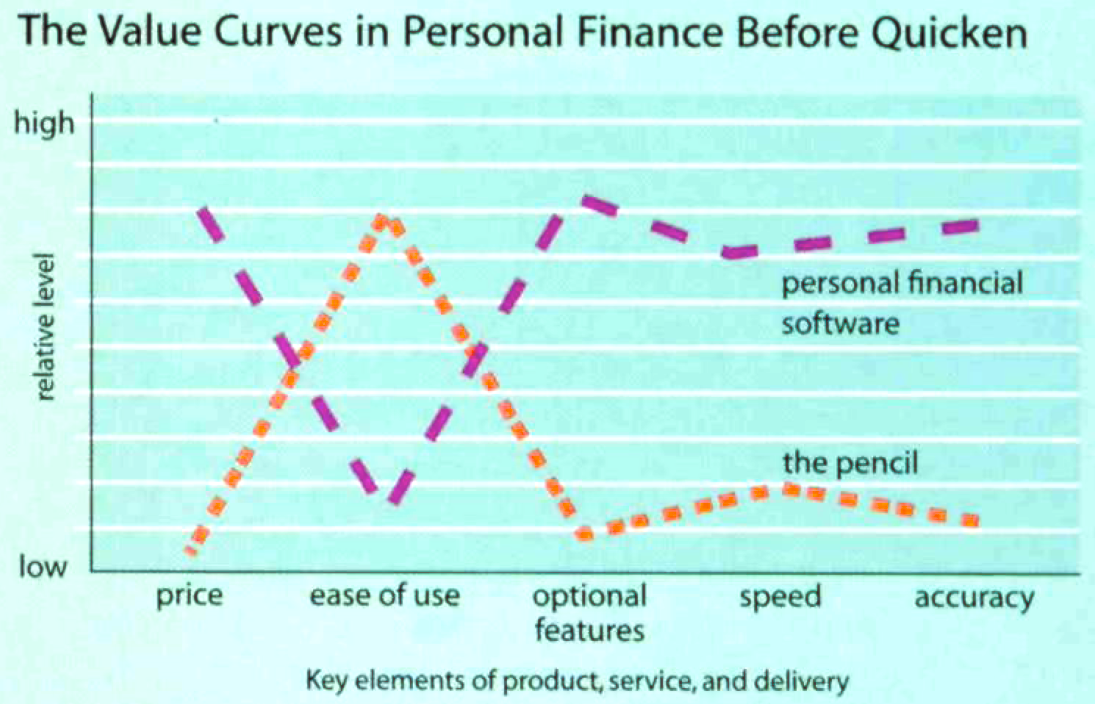
\includegraphics[width=4.5in]{curve.png}
\end{center}

The idea is to use this picture to realize new areas of the market that aren't filled.  Intuit used this type of idea to invent Quicken.  Nobody used optional features, computer software cost too much and was too hard to use.  So, remove extras, use a bunch of simple formulas, make the program really easy-to-use, and make it cheap (which is facilitated by removing features.)  Then you get speed and accuracy, which people love, and ease of use that rivals a pencil.  The key insight was recognizing that financial software doesn't compete against other software, but against the pencil.

The dimensions the authors say are good use to break through mental barriers are:

\begin{enumerate}
\item \textbf{Substitute Goods.}  The pencil vs. Quicken.
\item \textbf{Complementary Goods.}  The iPod and iTunes fulfilled extremely complementary needs, and thus dominated the competition.  This was as opposed to the Sansa, which isn't associated with software and so has always sucked.
\item \textbf{Product Scope.}  Barnes and Noble succeeded in the 1990's by thinking about bookstores as more than just places to buy books.  Instead, it was also a place to \textit{read} books, as well as relax and even eat.  Going the other direction, Jony Ive realized that iMacs and Macbooks don't need DVD drives all that badly.  A reduction in product scope was an innovation.
\item \textbf{Strategic Groups.}  Polo took elements from high-end clothing and elements from low-end clothing and got the best of both worlds.  Notice, Lauren ended up charging a premium price, not a mid-range price.  That is, he didn't average things, he went with a mix of extremes.  Sony mixed the coolness of the boom-box with the portability of the transistor radio to get the super successful Walkman.
\item  \textbf{The Chain of Buyers.}  Reuters catered to IT managers, and Bloomberg came in and catered to traders and CFO's.  Buyers as opposed to users, in this case.  
\item   \textbf{Functional vs. Emotional}  Swatch turned a previously functional item, where the competition had been about quartz accuracy and easy to read displays, into a fashion accessory.  It tells the time and it looks good, so people bought 5 or 6 of them to match different outfits.  
\end{enumerate}

A figure to wrap up:

\begin{center}
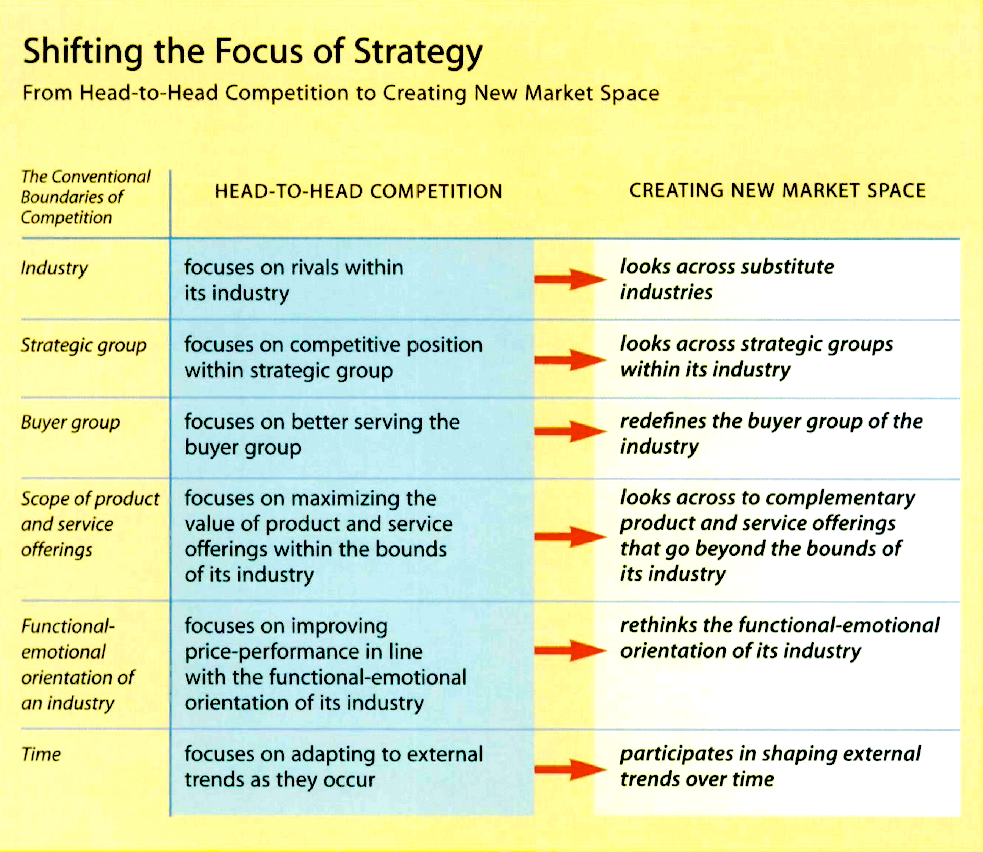
\includegraphics[width=4in]{wrapup.png}
\end{center}
One big point of all this is that people get stuck on a few dimensions, like price and speed.  You want to give the most speed for the cheapest price, and then you get stuck in a competitive deathtrap.  The ideas above can be used to think of new dimensions for the product.  The hard part is that everyone gets trained to think about the prominent dimensions of a given product and never even ventures out.  What is needed in conjunction with these ideas is a routine way to apply them.  Maybe just monthly, you apply this article to what you're doing.  


\end{document}  
